%
% Temporal databases
%
A \emph{temporal database}~\cite{etzion1998} is a database that manages some aspects of time in its schema~\cite{Dyreson1994}. The reality a temporal database tries to model, contains some temporal notions which have to be handled specifically in order to maintain a consistent modelling behavior. A very extensive list with the most well-known models in temporal databases can be found in ~\cite{Yu1998}. Nevertheless, it is necessary to define some consistent way to query the temporal data. There are several languages for querying temporal databases like TSQL~\cite{TSQL}. In~\cite{Snodgrass98} a proposal to add temporal support to the standard SQL is given.


\begin{svgraybox}
The temporal notions in temporal databases can be classified into the following types based on their interpretation and modelling purpose. User-defined time has no interpretation, but the other types do:\\

	\textbf{Transaction time} \emph{TT}~\cite{Jensen:1991:IIM:627283.627484}: The time when the fact is stored in the database.\\
	
	\textbf{Valid time} \emph{VT}~\cite{Snodgrass:1984:TQL:588011.588041}: The time when the fact is true in the modelled reality.\\
	
	\textbf{Decision time} \emph{DT}~\cite{Nascimento95}: The time when an event was decided to happen. \\
\end{svgraybox}
	
Database models can also be classified into \emph{bi-temporal} (both valid and transaction-time) or \emph{tri-temporal}  (bi-temporal and decision time) models.



\subsection{\label{subsubsec:primary-key}Primary key on temporal databases}
One of the first tasks in the design of a database is the choice for the primary key. In a temporal database, the most common solution for the choice of the primary key is to extend the primary key with the temporal value. Nevertheless, when dealing with uncertainty in the temporal values, the solution is usually to create a version identifier otherwise the primary key have uncertainty which should be avoided.

The following example illustrates the case of a table from a valid time database.

\begin{example}
\label{ex:pk}
Consider the following example database in \ref{table:example-database}. It contains regular data from employees in a company like the name, the birth date. Also two temporal values which represent a valid-time interval. Consider now that we want to hire Sarah again. That is not possible because of the primary key (ID) does not allow to insert again the row Sarah but with a different start and end time. In some models this is resolved by adding to the primary key both values Start and End years. The resulting database allows to insert a new row where Sarah the year 2010. But this modification also allows to insert spurious values e.g. inconsistent time periods (see last row in table \ref{table:example-database-with-new-pk}).


%\vspace{-10pt}

\begin{table}
\centering
\caption{Example database}
\begin{tabular}{c c c c c c }
\hline
\textbf{ID} & \textbf{Name} & \textbf{Age} & \textbf{Works for} & \textbf{Start year} & \textbf{End year} \\ \hline
1 & Peter & 24 & John &  2010 & - \\
2 & Maria & 34 & John & 2001 & - \\
3 & John & 52 & - &  1999 & - \\
4 & Sarah & 29 & Maria &  2005 & 2009 \\
\hline 
\end{tabular}
\label{table:example-database}

%\vspace{10pt}


\end{table}

%\vspace{-25pt}


%\vspace{-10pt}

\begin{table}
\centering
\caption{Example database with new primary key and some spurious values}
\begin{tabular}{c c c c c c }
\hline
\textbf{ID} & \textbf{Name} & \textbf{Age} & \textbf{Works for} & \textbf{Start year} & \textbf{End year} \\ \hline
1 & Peter & 24 & John &  2010 & - \\
2 & Maria & 34 & John & 2001 & - \\
3 & John & 52 & - &  1999 & - \\
4 & Sarah & 29 & Maria &  2005 & 2009 \\
4 & Sarah & 29 & Maria &  2010 & - \\
4 & Sarah & 29 & Maria &  2007 & 2008 \\
\hline 
\end{tabular}
\label{table:example-database-with-new-pk}

%\vspace{10pt}


\end{table}

%\vspace{-25pt}

\end{example}

\subsection{\label{subsubsec:consistency}Consistency on temporal databases}
The consistence mechanism in a temporal database is usually re-defined. The main problem is the insertion of spurious values in the database, as shown in example \ref{ex:pk}, in table \ref{table:example-database-with-new-pk}. The most usual solution is to re-define the DML (\emph{Data Manipulation Language}). e.g. the \emph{update} sentence is redefined as two sentences an update and a create sentence as illustrated in the following example.

\begin{example}
Consider the database in table \ref{table:example-database}. The following \emph{update} sentence:

\begin{verbatim}
Update Employees set StartYear = 2010 where ID=3;
\end{verbatim}

Is translated into the following two sentences: an update for the last version of the row and an insert sentence for the new version. The update sentence showed above is translated into:

\begin{verbatim}
Update Employees set EndYear = 2010 where ID=3;
Insert into Employees values (3,John,52,-,2010,-);
\end{verbatim}

%\vspace{-10pt}

\begin{table}
\centering
\caption{Example database after update sentence}
\begin{tabular}{c c c c c c }
\hline
\textbf{ID} & \textbf{Name} & \textbf{Age} & \textbf{Works for} & \textbf{Start year} & \textbf{End year} \\ \hline
1 & Peter & 24 & John &  2010 & - \\
2 & Maria & 34 & John & 2001 & - \\
3 & John & 52 & - &  1999 & 2010 \\
3 & John & 52 & - &  2010 & - \\
4 & Sarah & 29 & Maria &  2005 & 2009 \\
\hline 
\end{tabular}
\label{table:example-database-update}

%\vspace{10pt}


\end{table}

%\vspace{-25pt}

Table \ref{table:example-database-update} shows the resulting database after the update sentence.

\end{example}


\subsection{Commercial Temporal database systems}
There are several commercial temporal DBMS. Table \ref{table:commercial-temporal-db} is a comparative among the most well-known systems. It is also provided a reference for more information. 

Oracle workspace manager~\cite{oracle2009} and TimeDB~\cite{timedb2005} are libraries for dealing with time in an OracleDB. Nevertheless TimeDB and Postgree Temporal~\cite{posgree2009} are similar. Both are simple implementations that implement a subset of the Allen's operators and some operations for the creation and manipulation of a temporal attribute (valid, transaction or both times) in a table. Nevertheless, Teradata~\cite{teradata2011} is mainly a business intelligence database designed for data-mining. 

The most complete implementation is the Workspace Manager, which is described briefly in the following section. Unfortunately, none of these systems work with uncertainty or imprecision neither in the data storage nor in the query.

\begin{table}
\centering
\caption{Commercial implementations for temporal database systems. }
\begin{tabular}{c c c c c c }
\hline
\textbf{Name} & \textbf{Time managed} & \textbf{Comments} & \textbf{References}  \\ \hline
Oracle Workspace Manager & VT and TT. & Package for Oracle DB. & \cite{oracle2009}\\
TimeDB & VT and TT. & Interface for Oracle DB. & \cite{timedb2005}\\
Postgree Temporal & VT. & Package for Postgree SQL. & \cite{posgree2009}\\
Teradata & VT and TT. & Used for data-mining. & \cite{teradata2011}\\
\hline 
\end{tabular}
\label{table:commercial-temporal-db}

%\vspace{10pt}


\end{table}

\subsubsection{Oracle Workspace Manager}

\begin{figure}
\centering
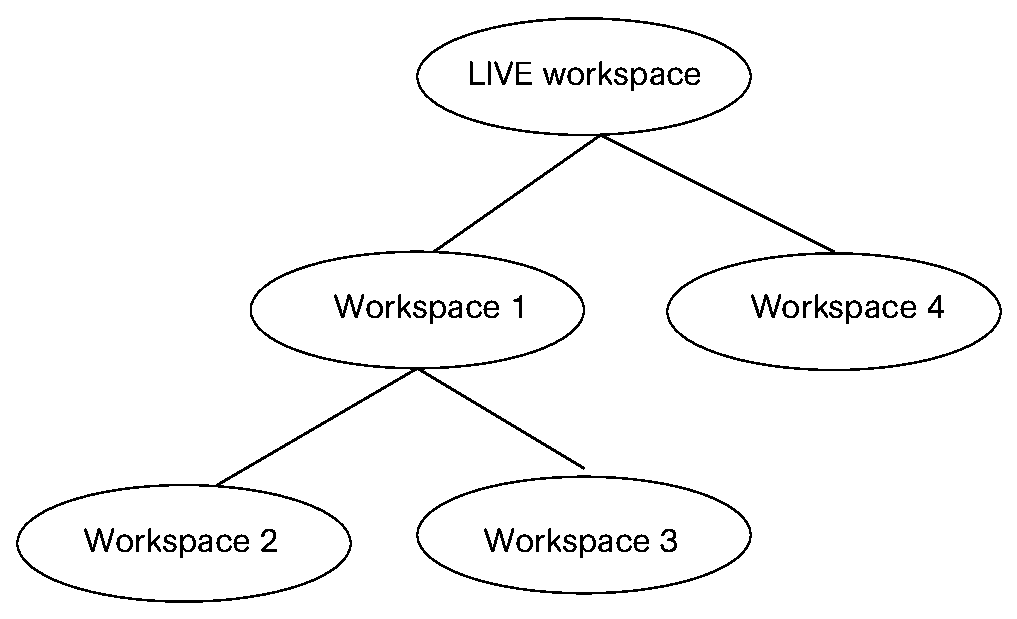
\includegraphics[scale=0.5]{graphs/workspaceTopology.eps}
\caption{A sample topology in the workspace manager.}
\label{fig:workspace-topology}
\end{figure}

Oracle workspace manager \cite{OraE118602} package allows to get several versions of the data in the same database. It is also possible to version only a table. The main benefits of this are two:

\begin{itemize}
\item
Organization and optimization of data in a hierarchical frames: It is possible to create a frame of time (a workspace) and work only with that partial version of the data. It is provided a mechanism to merge data among different workspaces and to solve conflicts. The organization of data in these workspaces for very large tables result in smaller time access.
\item
Valid time as well as transaction time are managed by the system. Each update sentence makes a change in the versioning of a row.
\end{itemize}

When a table is versioned, the system creates a few tables and views as well as auxiliary structures to allow keep several version of the data, while keeping the primary key defined by the user.

A workspace is a logical group of a set of changes (versions of tuples) and allows consistent access, thus the user always obtain the correct data version. Workspaces are ordered in a hierarchy. The top level is called LIVE workspace (see figure \ref{fig:workspace-topology}).  \\

The system only makes a copy of a tuple if it is changed. In order to access different versions of the tuple, the context must be changed. Also, it is not necessarily to modify the SQL code to access to versioned tables.\\
%When a table is versioned, it is renamed as table\_LT. Here is stored all the data for the information together metadata for the versioning. An auxiliary table is created with the workspace metadata with the name table\_AUX. A view is created with the name of the original table to allow querying without versioning.

